% Fig. 3.15 -- 獨立性一篇的聯合值域圖。
% 書稿來源: mathstatch3.tex 第 1834 至 1871 行的 tikzpicture。
% 書稿以 gray、opacity 0.2 填色, 網頁改 journalaccent、透明度 0.15。
% 幾何與比例尺沿用同一個三角形值域的 triangle-range-integration.tex (Fig. 3.4),
% 兩張圖畫的是同一個聯合值域, 併排比較時字級與線寬一致。
\documentclass[tikz,border=2pt]{standalone}
\usepackage{amsmath}
\usepackage{amssymb}
\usepackage{xcolor}

\definecolor{journalink}{HTML}{1F1C18}
\definecolor{journalmuted}{HTML}{8A7F72}
\definecolor{journalaccent}{HTML}{9C2D2D}

\begin{document}
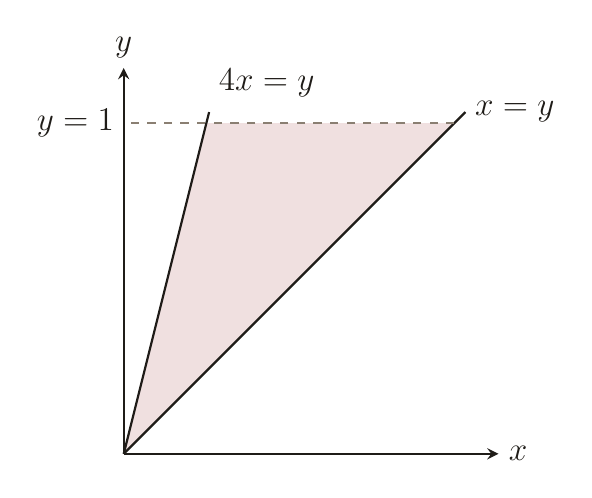
\begin{tikzpicture}[x=1.4cm, y=1.4cm, >=stealth,
                    every node/.style={journalink, font=\large}]

  %% 聯合值域 0 < x < y < 1 之中 4x > y 的那一塊
  %% 三個頂點分別是原點、直線 x=y 與 y=1 的交點、直線 4x=y 與 y=1 的交點
  \fill[journalaccent, fill opacity=0.15]
    (0,0) -- (3,3) -- (0.75,3) -- cycle;

  %% 值域的右界 x = y
  \draw[journalink, line width=0.8pt] (0,0) -- (3.1,3.1);
  \node[journalink, right] at (3.1,3.1) {$x=y$};

  %% 分界線 4x = y
  \draw[journalink, line width=0.8pt] (0,0) -- (0.775,3.1);
  \node[journalink, above right, yshift=2pt] at (0.775,3.1) {$4x=y$};

  %% 值域的上界 y = 1
  \draw[journalmuted, line width=0.5pt, dashed] (3,3) -- (0,3);
  \node[journalink, left] at (0,3) {$y=1$};

  %% 座標軸
  \draw[journalink, line width=0.8pt, ->] (0,0) -- (3.4,0) node[right] {$x$};
  \draw[journalink, line width=0.8pt, ->] (0,0) -- (0,3.5) node[above] {$y$};

\end{tikzpicture}
\end{document}
